\documentclass[a4paper,12pt]{article}
\usepackage[T1]{fontenc}
\usepackage{amsmath}
\usepackage{graphicx}
\usepackage{geometry}
\usepackage{noto}
\usepackage{microtype}
\usepackage{hyphenat}
\usepackage{float}
\usepackage{graphicx}
\usepackage{caption}
\usepackage{float}
\geometry{margin=1in}

\hyphenation{fre-quên-cias fi-ltro si-nais aten-ua-ção}

\begin{document}
	
	% Cover page
	\begin{titlepage}
		\centering
		\vspace*{2cm}
		\Huge
		\textbf{Trabalho Prático de PDS do Capítulo 7} \\
		\vspace{1cm}
		\Large
		Leonardo Santos \\
		Universidade Federal do Paraná \\
		\vspace{0.5cm}
		\normalsize
		\vspace{2cm}
		
\includegraphics[width=0.5\textwidth]{ufpr.png} \\
		\vspace{1cm}
		\large
		Professor: Gideon \\
		Curso: Processamento Digital de Sinais \\
		Cidade: Curitiba \\
		Data: julho de 2025 \\
	\end{titlepage}
	
	\section{Introdução}
	Em sinais de voz, é comum a presença de ruídos de fundo que dificultam a inteligibilidade. O uso de filtros digitais permite isolar frequências relevantes e atenuar componentes indesejadas. Neste experimento, aplicamos filtros FIR (Finite Impulse Response) e IIR (Infinite Impulse Response), ambos do tipo passa-faixa, visando reter a faixa de 400 Hz a 600 Hz, que contém parte importante do conteúdo vocal.
	
\section{Materiais e Métodos}

Foi utilizado um sinal de voz com ruído de fundo, previamente gravado e carregado no ambiente Python por meio da biblioteca \texttt{scipy.io.wavfile}. A gravação foi convertida para ponto flutuante e normalizada, garantindo compatibilidade com os algoritmos de filtragem digital.

O projeto do filtro FIR foi realizado utilizando a função \texttt{firwin}, com 101 coeficientes e janela de Hamming, configurado como passa-faixa na faixa de 400 Hz a 600 Hz. Já o filtro IIR foi do tipo Butterworth, de quarta ordem, implementado com a função \texttt{butter}, também na configuração passa-faixa para a mesma faixa de frequências.

Ambos os filtros foram aplicados ao sinal com o uso das funções \texttt{lfilter} e \texttt{filtfilt}, sendo esta última empregada no filtro IIR para eliminar distorções de fase e transientes de borda. As análises foram conduzidas no domínio do tempo, da frequência e da fase, e todas as figuras foram geradas com a biblioteca \texttt{matplotlib}.

A Figura~\ref{fig:orig_plot} apresenta o sinal original no tempo e seu espectro de magnitude, obtido por meio da Transformada Rápida de Fourier (FFT). Esta análise espectral foi essencial para estimar a faixa de interesse (400 Hz a 600 Hz), que guiou a definição das bandas de corte utilizadas nos filtros projetados.

\begin{figure}[!htbp]
	\centering
	\captionsetup{skip=0pt}
	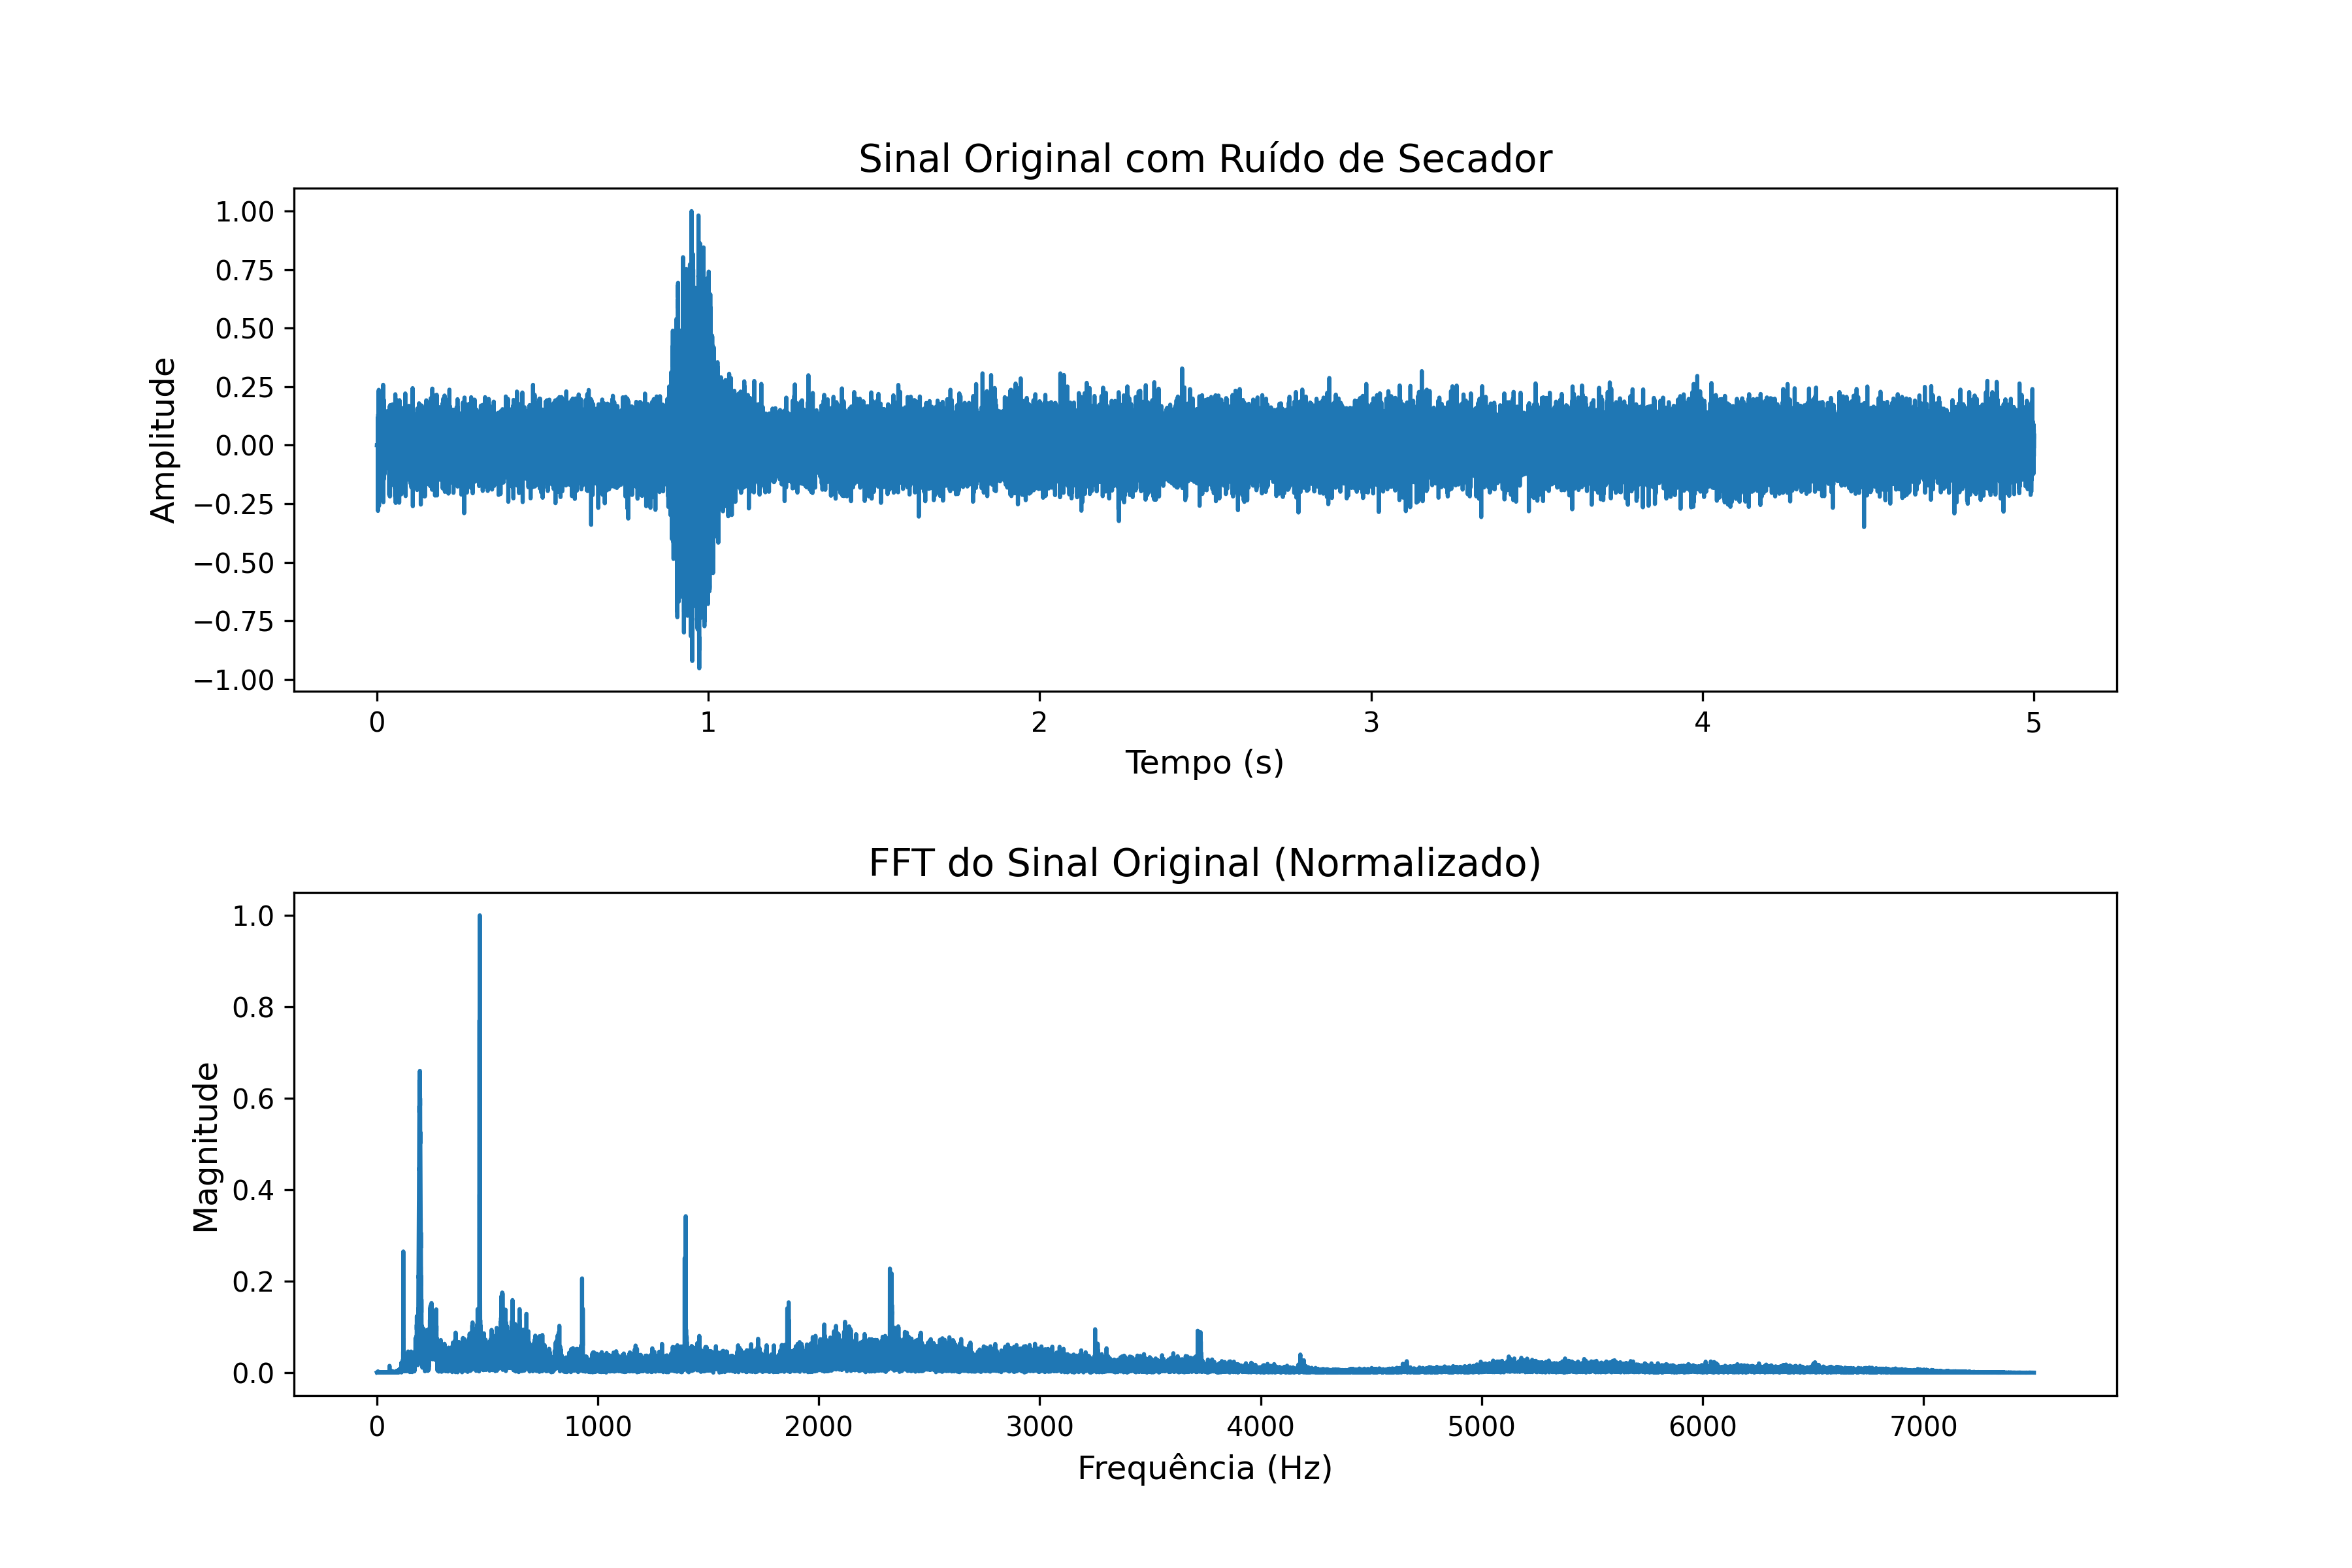
\includegraphics[width=\textwidth,height=0.8\textheight,keepaspectratio]{original_plot.png}
	\caption{Sinal original e sua Transformada de Fourier (FFT).}
	\label{fig:orig_plot}
\end{figure}

	
	\section{Resultados}
	
	\subsection{Sinal Filtrado com FIR}
	A Figura~\ref{fig:fir_plot} mostra o sinal após filtragem FIR. Observa-se que o ruído foi significativamente atenuado fora da banda de 400–600 Hz, preservando as componentes principais da voz.
	
	\begin{figure}[!htbp]
		\centering
		\captionsetup{skip=0pt} % Reduz espaço entre imagem e legenda
		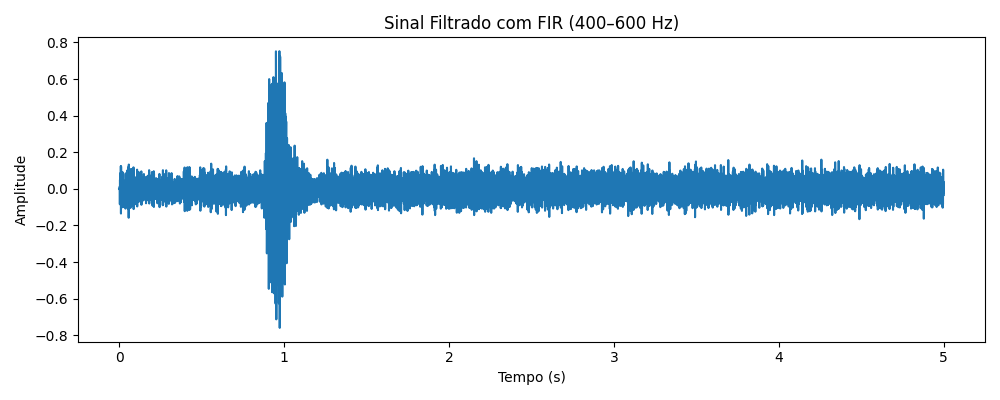
\includegraphics[width=\textwidth,height=0.8\textheight,keepaspectratio]{fir_plot.png}
		\caption{Sinal filtrado com filtro FIR (400–600 Hz).}
		\label{fig:fir_plot}
	\end{figure}
	\subsection{Sinal Filtrado com IIR}
	A Figura~\ref{fig:iir_plot} apresenta o resultado da filtragem com o filtro IIR. A atenuação do ruído também foi eficiente, preservando a mesma faixa de interesse. O uso de \texttt{filtfilt} garantiu boa estabilidade e evitou transientes no início do sinal.
	
	\begin{figure}[!htbp]
		\centering
		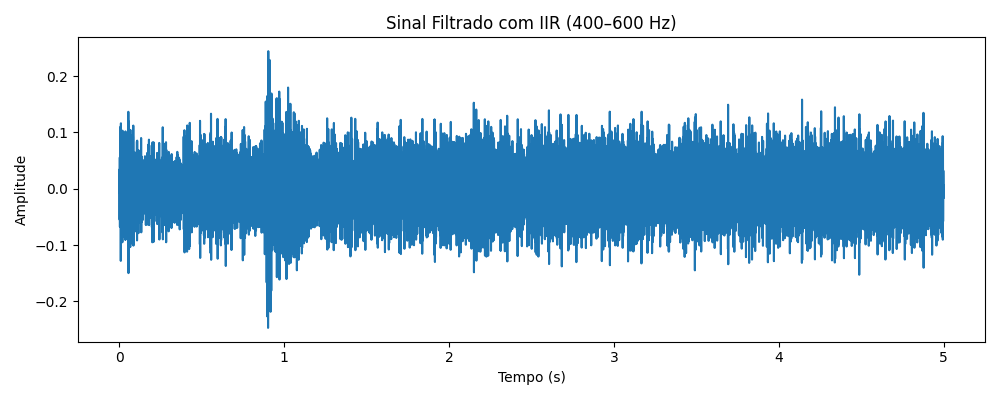
\includegraphics[width=\textwidth,height=0.8\textheight,keepaspectratio]{iir_plot.png}
		\caption{Sinal filtrado com filtro IIR (400–600 Hz).}
		\label{fig:iir_plot}
	\end{figure}
	
	\subsection{Análise Espectral}
	A Figura~\ref{fig:fft_comparacao} mostra a comparação espectral dos sinais original, FIR e IIR. Nota-se que ambos os filtros atenuaram eficazmente as frequências fora da faixa desejada, com resultados bastante similares.
	
	\begin{figure}[!htbp]
		\centering
		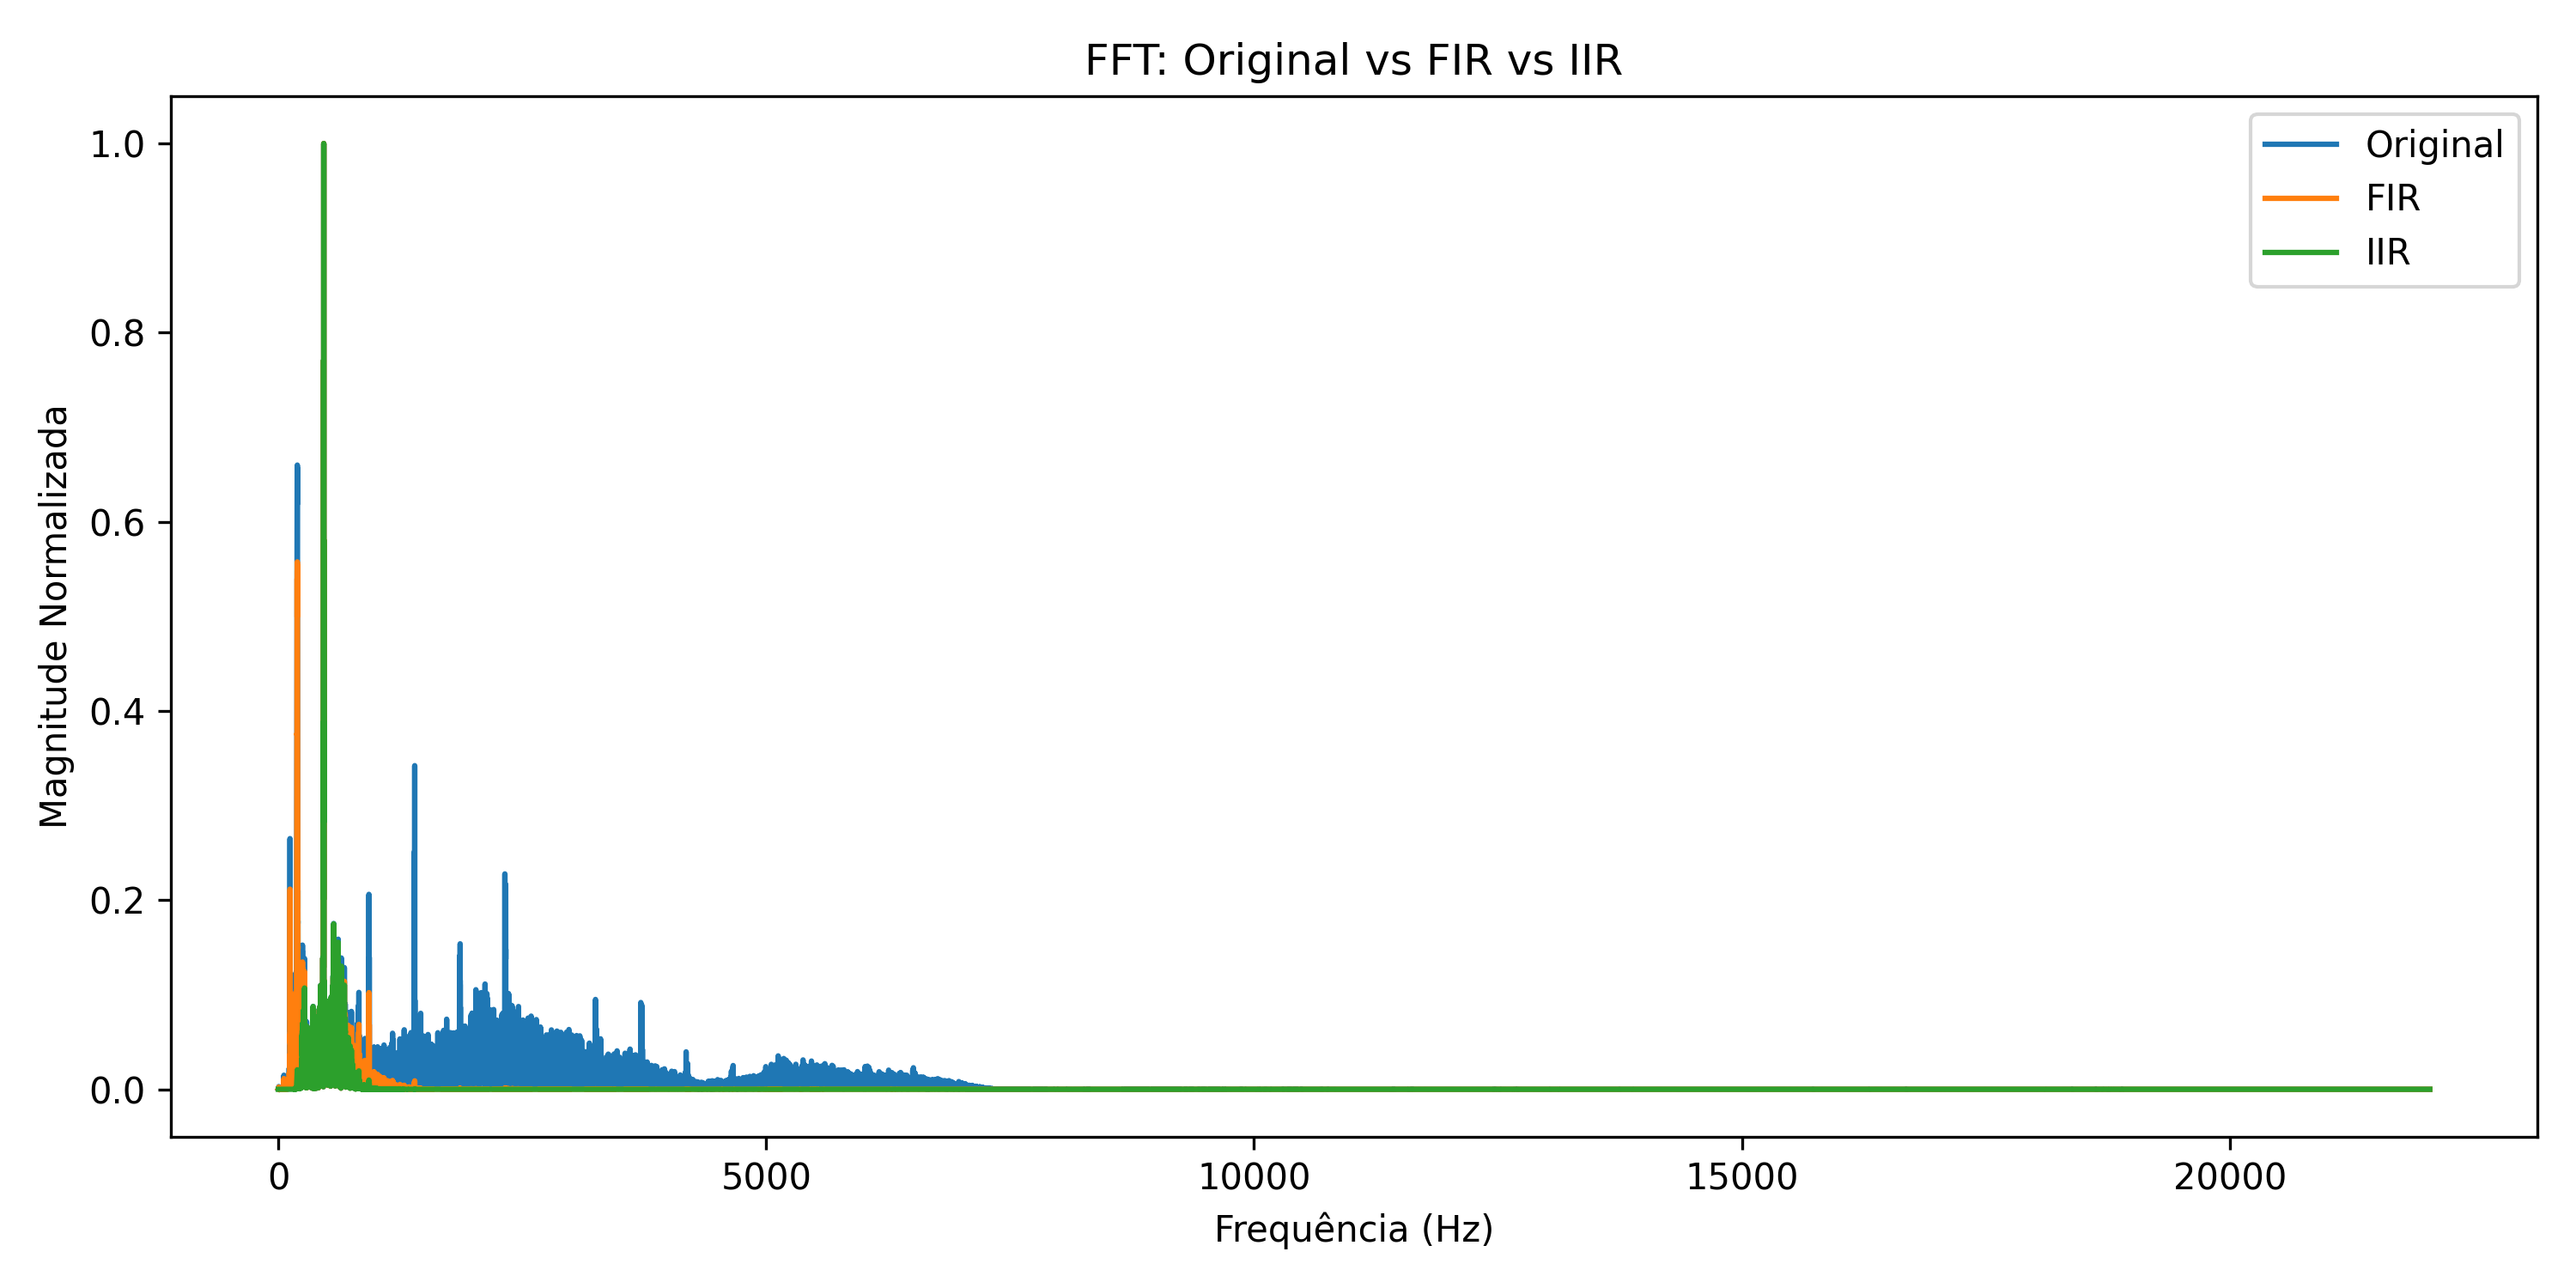
\includegraphics[width=\textwidth,height=0.8\textheight,keepaspectratio]{fft_comparacao.png}
		\caption{FFT do sinal original, filtrado com FIR e IIR.}
		\label{fig:fft_comparacao}
	\end{figure}
	
	\subsection{Resposta em Fase}
	A Figura~\ref{fig:fase_plot} compara as fases dos filtros. O FIR apresenta fase linear, o que é desejável em aplicações de áudio, enquanto o IIR apresenta distorção de fase, característica de filtros recursivos.
	
	\begin{figure}[!htbp]
		\centering
		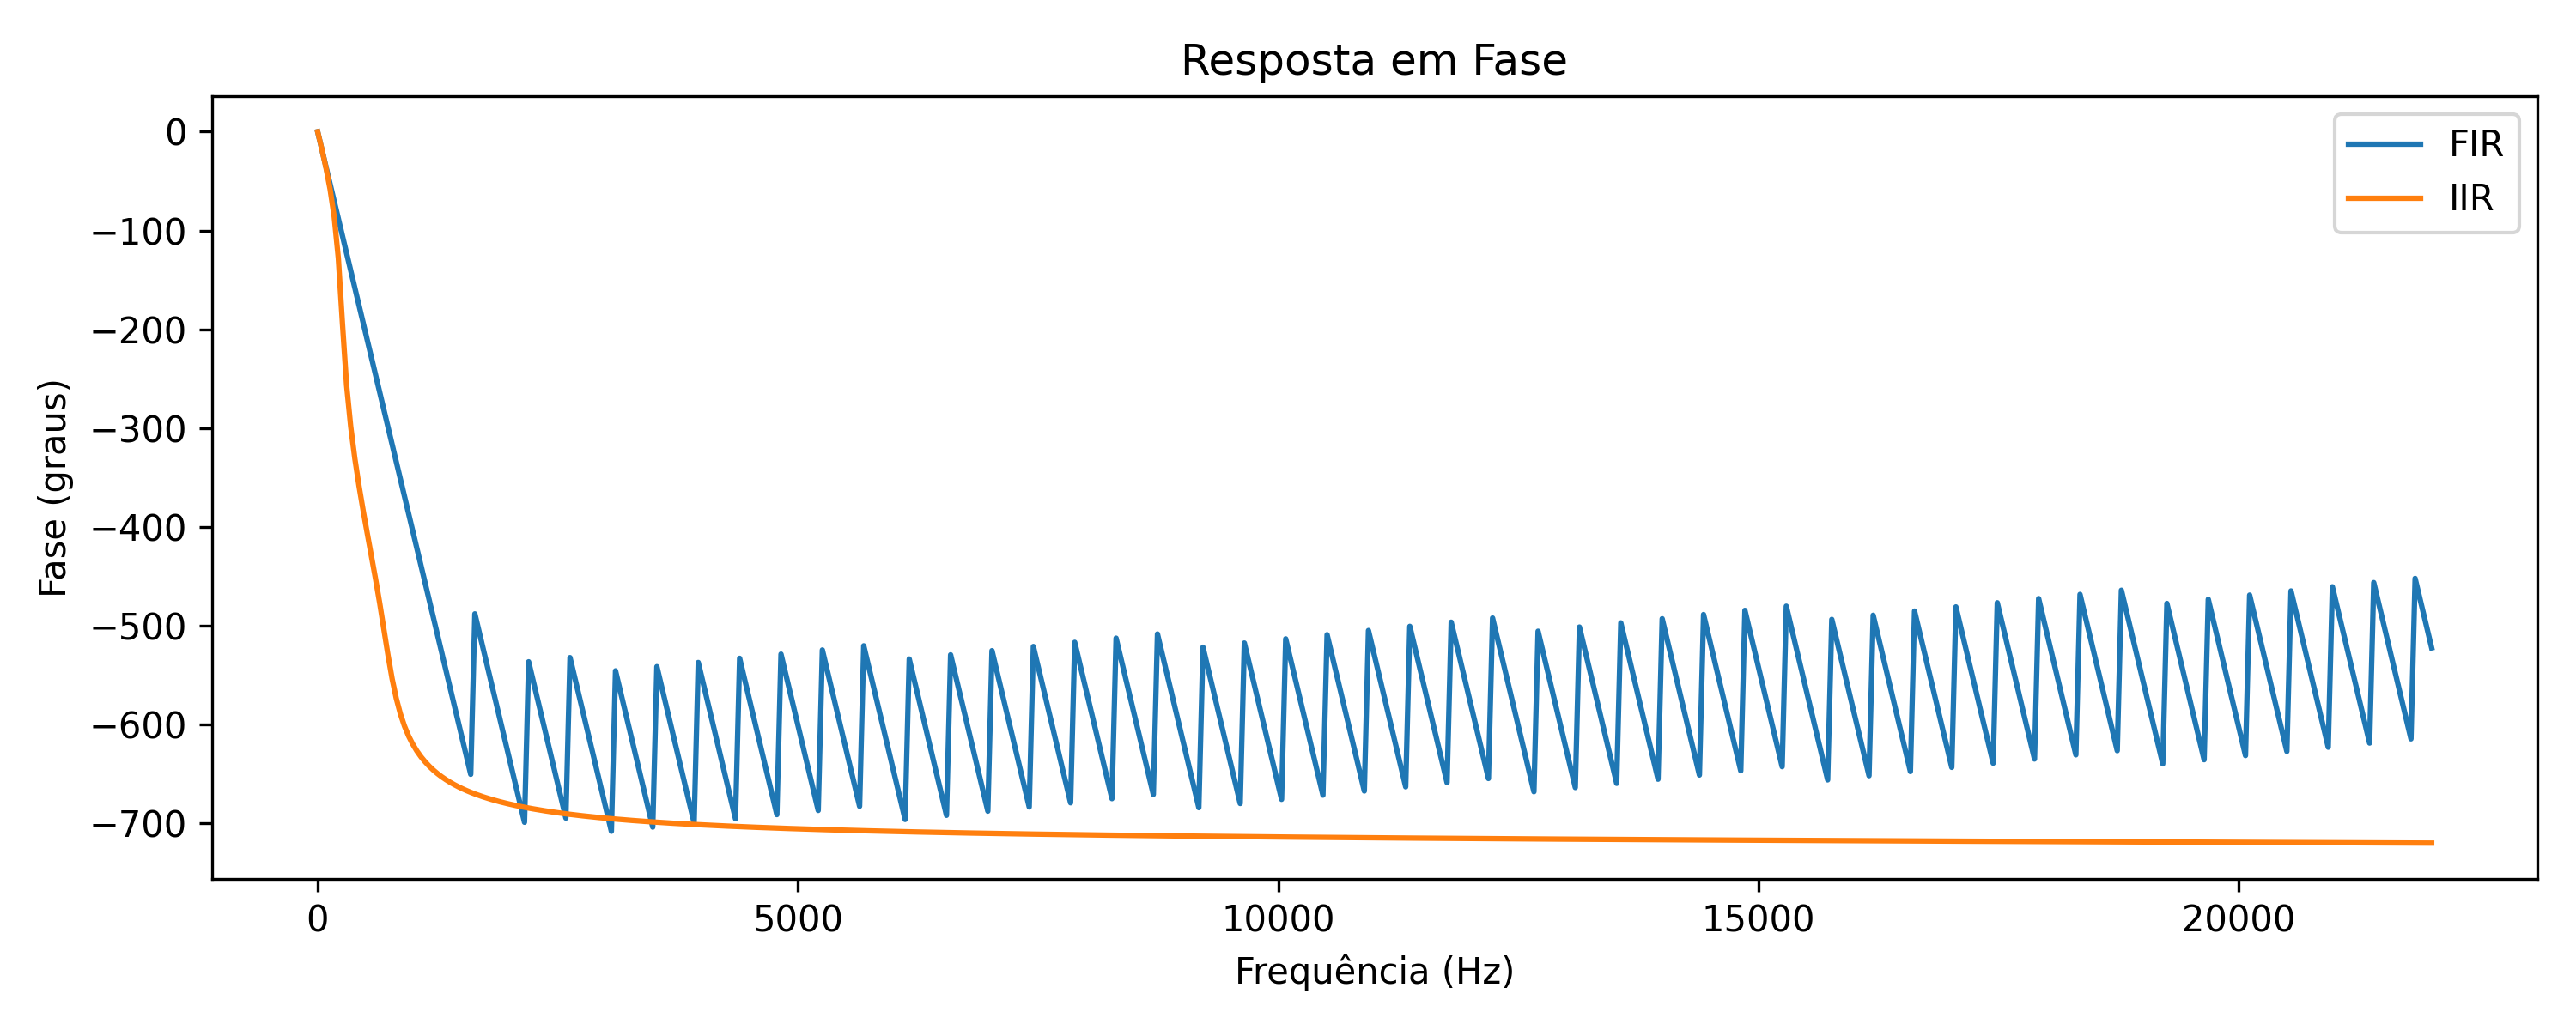
\includegraphics[width=\textwidth,height=0.8\textheight,keepaspectratio]{fase_fir_iir.png}
		\caption{Resposta em fase dos filtros FIR e IIR.}
		\label{fig:fase_plot}
	\end{figure}
	
	\section{Conclusão}
	Os filtros FIR e IIR projetados mostraram-se eficazes na atenuação de ruído fora da faixa de 400–600 Hz. O FIR apresentou melhor comportamento de fase (linear), sendo ideal para preservar a forma de onda original. O IIR, por sua vez, alcançou resultado similar com menor ordem, sendo mais eficiente computacionalmente, porém com distorção de fase. Ambos são viáveis conforme os requisitos da aplicação.
	
	
	
\end{document}